\documentclass[10pt]{article}
%\usepackage[utf8]{inputenc}
\oddsidemargin=0cm
\textwidth=15cm
\usepackage{graphicx}
%\usepackage[utf8x]{inputenc}
%\usepackage[spanish]{babel}
%\DeclareGraphicsExtensions{.bmp,.jpg}
\usepackage[latin1]{inputenc}
\usepackage{amsmath}
\usepackage{amsthm}
\usepackage{amsfonts}
\usepackage{adjustbox}
\usepackage{amssymb}
\usepackage[dvips]{epsfig}
\usepackage{ulem}
\usepackage{indentfirst}
\usepackage{wasysym}
\usepackage{pifont}
\usepackage{fancyhdr}
%\usepackage{color}
\usepackage{multicol}
\usepackage{framed}
\usepackage[usenames, dvipsnames]{color}
\usepackage{wrapfig}

%\textwidth=17cm %ancho del texto, de paso define margen de la derecha
%\topmargin=2cm %margen superior
%\oddsidemargin=-0.5cm %margen de la izquierda del texto
%\evensidemargin=0.5cm 

%\definecolor{color1}{RGB}{220,250,250}
\definecolor{shadecolor}{RGB}{220,250,250}
%238
\pagestyle{myheadings}
\definecolor{color1}{RGB}{220,250,250}
\definecolor{color2}{rgb}{0.99,0.9,1.0}
\definecolor{color3}{RGB}{220,250,250}
\definecolor{color4}{rgb}{0.0,0.5,0.69}
\definecolor{color5}{rgb}{1.0,1.0,0.88}
\definecolor{color6}{rgb}{1.0,0.94,0.84}
\definecolor{color7}{rgb}{0.94,1.0,1.0}
\definecolor{color8}{rgb}{1.0,0.94,0.84}
\definecolor{color9}{rgb}{0.0,0.5,0.69}
\definecolor{dblue}{rgb}{1.0,0.0,1.0}
\definecolor{dred}{rgb}{1.0,0.0,0.0}
\definecolor{lred}{rgb}{0.82,0.1,0.26}

%HIGHLIGHT 2 (turquise)
\newcommand{\2}[1]{\hspace{-0.93cm}\colorbox{color1}{\hspace{0.07cm} \parbox{17cm}{\vspace{0.2cm} #1}\hspace*{0.07cm} }}

%HIGHLIGHT 3 ()
\newcommand{\3}[1]{\hspace{-0.93cm}\colorbox{color7}{\hspace{0.07cm} \parbox{17cm}{\vspace{0.2cm} #1}\hspace*{0.07cm} }}
%NOTA
\newcommand{\nota}[1]{\textbf{Notaci\'on:}\: 
#1}

%LINE
\newcommand{\start}{\noindent {\color{color4}\rule{17cm}{0.5mm}}\\}

%Notation
\newcommand{\notation}[1]{\begin{framed}\noindent \nota{#1} \end{framed}}

%COMIENZO
\newcommand{\com}[1]{\noindent\rule{17cm}{0.8mm}
\begin{center}
\textbf{{\Large #1}}
\end{center}
\noindent\rule{17cm}{0.8mm}\\
}

%DEMOSTRACION
\newcommand{\dem}{\noindent {\color{color4}\rule{17cm}{0.5mm}}\\ \negrita{\textbf{Demostraci\'on: }}} 


%REFLEXION
\newcommand{\reflexion}[1]{\2{\textbf{\underline{Reflexi\'on.}}\\

#1\\}\\ }

%NEGRITA
\newcommand{\negrita}[1]{{\color{color4}\textbf{#1}}}

\newcommand{\red}[1]{{\color{red}\textbf{#1}}}

%HIGHLIGHT
\newcommand{\highlight}[1]{\begin{shaded} #1 \end{shaded}}

%FRAME
\newcommand{\enmarcar}[1]{\begin{framed} #1 \end{framed}}


%OBSERVATION 
\newcommand{\obs}[1]{\textbf{Observati\'on:} #1}

%HIGHLIGHT 2
\newcommand{\Highlight}[1]{\hspace{-0.93cm}\colorbox{color9}{\hspace{0.07cm} \parbox{12.7cm}{\vspace{0.2cm} #1}\hspace*{0.07cm} }}

% DESAFIO
\newcommand{\Desafio}[1]{\noindent\rule{13.3cm}{0.4mm}\\
\Highlight{ #1
\vspace{0.3cm} }
\noindent\rule{13.3cm}{0.3mm}\\}

%OBSERVATION
\newcommand{\observation}[1]{\begin{framed} \obs{#1} \end{framed}}

%SOLUTION
\newcommand{\sol}{\noindent {\color{color4}\rule{13.3cm}{0.5mm}}\\ \negrita{\textbf{Soluci\'on: }}} 

%\markboth{}{Construcci\'on de Tesis}

%\title{Control 1 de Matem\'aticas 1}
%\author{Programa de Bachillerato. Universidad de Chile.}
%\date{Lunes 24 de Marzo, 2013}
\theoremstyle{theorem}
\newtheorem{teo}{\textbf{Teorema}}%[chapter]
\newtheorem{lema}{\textbf{Lema}}%
\newtheorem{defi}{\textbf{Definici\'on}}%[chapter]
\newtheorem{propi}{Propiedad}%[chapter]
\newtheorem{propir}{Propiedad Relevante}%[chapter]
\newtheorem{pro}{Proposici\'on}%[chapter]
\newtheorem{ax}{Axioma}
\newtheorem{prob}{Problema}
\newtheorem{eje}{Ejemplo}%[chapter]
\newtheorem{ejer}{\textsc{Ejercicio}}%[section]
\newtheorem{ejerr}{Ejercicio Resuelto}
\newtheorem{obser}{Observaci\'on}%[chapter]
\newcommand{\R}{\mathbb{R}} 
\newcommand{\Z}{\mathbb{Z}}
\newcommand{\Q}{\mathbb{Q}}
\newcommand{\C}{\mathbb{C}}
\newcommand{\N}{\mathbb{N}}
\newcommand{\U}{\mathbb{U}}
\newcommand{\D}{\mathbb{D}}
\newcommand{\I}{\mathbb{I}}
\numberwithin{equation}{section}
\pagestyle{myheadings}
\usepackage{enumerate}
\newcommand{\dis}{\displaystyle}
\usepackage[all]{xy}
\usepackage{tabu}  %paquete para hacer tablas

\title{C\'alculo Diferencial (MAT170)\\ Clase 6 }
\author{Prof. Marco Godoy\\
marco.godoy@edu.udla.cl}
\date{Abril 2019}

\begin{document}


\maketitle

\section{Trigonometr\'ia en el triangulo rect\'angulo}

\subsection{Las funciones trigonom\'etricas seno, coseno y tangente}
Considere el siguiente tri\'angulo rect\'angulo a continuaci\'on. Es posible estudiar las razones trigonom\'etricas en \'angulos $\alpha,\, \beta$ tales que: 
\begin{align*}
0&\leq\alpha\leq \frac{\pi}{2}\\
0&\leq\beta\leq \frac{\pi}{2}.\\ 
\end{align*}
Los lados opuestos a los \'angulos $\alpha$ y $\beta$ se llaman catetos, mientras que la \textbf{hipotenusa} es el lado opuesto al \'angulo $\dis \frac{\pi}{2}$ (representado por un cuadrado peque\~no donde va dicho \'angulo). Un cateto es \textbf{adyacente} u \textbf{opuesto} a un \'angulo, si como segmento forma parte de la abertura que define dicho \'angulo. Por ejemplo, en la Figura \ref{triangulorectangulo}, el lado $a$ es un cateto opuesto al \'algulo $\alpha$, mientras que $b$ es un cateto adyacente.
\input{fig_1.TpX}
Se definen las funciones trigom\'etricas a continuaci\'on:

\begin{align*}
seno &= \frac{cateto\, opuesto}{hipotenusa}\\
coseno &= \frac{cateto\, adyacente}{hipotenusa}\\
tangente &=\frac{cateto\, opuesto}{cateto\, adyacente}\\
\end{align*} 

\subsection{Otras funciones trigonom\'etricas}\label{otras_trigo}

Aparte de las funciones trigonom\'etricas seno, coseno y tangente, se definen las funciones trigonom\'etricas \textbf{secante}, \textbf{cosecante} y \textbf{cotangente} como: 
\begin{align*}
\sec(\alpha)&=\frac{1}{\cos(\alpha)}\\
\csc(\alpha)&=\frac{1}{\sin(\alpha)}\\
\cot(\alpha)&=\frac{1}{\tan(\alpha)}
\end{align*}
\section{Trigonometr\'ia en el c\'irculo unitario}

\subsection{Definici\'on y ejemplos}
Es posible estudiar las razones trigonom\'etricas en el \textbf{plano cartesiano}, mediante el c\'irculo unitario (c\'irculo de radio $1$), como se muestra en la Figura \ref{circulounitario}
\input{fig_2.TpX}
Es posible estudiar las razones trigonom\'etricas en \'angulos $\alpha,\, \beta$ tales que: 
\begin{align*}
0&\leq\alpha\leq 2\pi\\
0&\leq\beta\leq 2\pi.\\ 
\end{align*}

\begin{eje}
En la Figura \ref{ejemploangulos} algunos ejemplos.
\input{fig_3_pi4.TpX}
\end{eje}


\subsection{Extensi\'on de funciones trigonom\'etricas para \'angulos negativos}

Es posible extender el dominio de las funciones trigonom\'etricas seno y coseno a \'angulos negativos ocupando el c\'irculo unitario, de la siguiente manera como se muestra en la Figura \ref{angulosnegativos}. La diferencia est\'a es que ahora el \'angulo se mide en sentido \textbf{horario}, es decir, siguiendo el movimiento de las manecillas del reloj. Para saber el valor de las funciones seno y coseno con \'angulos negativos, ocuparemos el siguiente resultado:

\begin{pro}
Se cumplen las siguientes igualdades:
\begin{align*}
\sin(-\alpha)&= -\sin(\alpha)\\
\cos(-\alpha)&=\cos(\alpha)
\end{align*}
\end{pro}
\input{fig_4.TpX}

\begin{eje}
Calcule $\sin(-\pi/4)$ y $\cos(-\pi/4)$.
\\\\
\textbf{Desarrollo.}
\begin{align*}
\sin(-\pi/4)&=-\sin(\pi/4)=\sqrt{2}/2,\\
\cos(-\pi/4)&=-\cos(\pi/4)=\sqrt{2}/2,
\end{align*}
\end{eje}

\begin{obser}
El resto de las funciones trigom\'etricas: tangente, cotangente, secante y cosecante se calculan de la misma manera que en la Subsecci\'on \ref{otras_trigo}.
\end{obser}

\newpage
\section{Problemas propuestos}

\begin{enumerate}
  \item Ocupando el tri\'angulo rect\'angulo, resuelva los siguientes problemas:
     \begin{enumerate}[1.]
         \item Si $\alpha =60^{o}$, $c=13$. Calcule $a$ y $b$.
         \item Si $\alpha =45^{o}$, $c=15$. Calcule $a$ y $b$.
         \item Si $\dis \beta =\frac{\pi}{6}$, $a=5$. Calcule $b$ y $c$.
         \item Si $\beta =50^{o}$, $b=8$. Calcule $a$ y $c$.
         \item Si $a=3$, $b=4$. Calcule $\alpha$, $\beta$. Exprese su resultado en grados sexagesimales y en radianes. 
     \end{enumerate}
  \item Desde la parte superior de un edificio, que mide $100$ pies de altura, un
hombre observa un autom\'ovil que se desplaza frente al edificio (Figura \ref{auto}). Si el \'angulo de
depresi\'on del autom\'ovil cambia de $46^{o}$ a $22^{o}$ durante el periodo de observaci\'on,
cu\'anto se ha trasladado el autom\'ovil?
\begin{figure}[h]\label{auto}
\centering
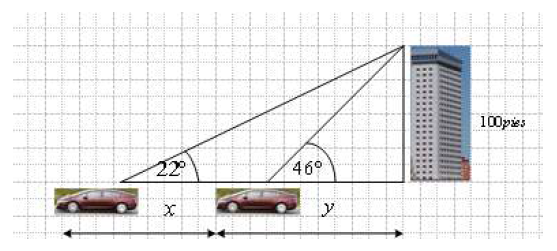
\includegraphics[scale=0.5]{fig_3}
\end{figure}
  \item Ocupando el c\'irculo unitario y las definiciones de las funciones trigonom\'etricas, resuelva lo siguiente:
\begin{enumerate}[1.]
   \item Demuestre que $\sin^2(\alpha)+\cos^2(\alpha)=1$.
   \item Demuestre que $\tan^2{\alpha}+1=\sec^2(\alpha)$.
   \item Demuestre la siguiente identidad trigonom\'etrica: $$\frac{\cos(\alpha)}{1+\sin(\alpha)}+\frac{1+\sin(\alpha)}{\cos(\alpha)}=2\sec(\alpha).$$
\end{enumerate}




\end{enumerate}


\end{document}